% CIFAR-10 RGB-bit-exact bpd baselines 对比柱状图
% 编译: pdflatex baselines.tex   (或 latexmk -pdf)
% 嵌入论文: % CIFAR-10 RGB-bit-exact bpd baselines 对比柱状图
% 编译: pdflatex baselines.tex   (或 latexmk -pdf)
% 嵌入论文: % CIFAR-10 RGB-bit-exact bpd baselines 对比柱状图
% 编译: pdflatex baselines.tex   (或 latexmk -pdf)
% 嵌入论文: % CIFAR-10 RGB-bit-exact bpd baselines 对比柱状图
% 编译: pdflatex baselines.tex   (或 latexmk -pdf)
% 嵌入论文: \input{figures/baselines.tex}
%
% 数据来源: README.md L27-35 (RGB-bit-exact 同域可比)
%   PixelCNN++         ~53.5M 2.92    Salimans et al., ICLR 2017  (公开 ~53.5M; 脚本核算锚 55.35M, 见 scripts/pixelsnail_paramcount.py)
%   Image Transformer  ~40M   2.90    Parmar et al., ICML 2018  (原文未报告参数量; ~40M 据官方 tensor2tensor imagetransformer_cifar10_base = 12L/d512/ff2048 估算)
%   PixelSNAIL         ~91M   2.85    Chen et al., ICML 2018  (原文未报告参数量; ~91M 据官方 neocxi/pixelsnail-public CIFAR 配置 h12_noup_smallkey/nr_filters=256/nr_resnet=4 核算, 见 scripts/pixelsnail_paramcount.py)
%   Sparse Transformer  59M   2.80    Child et al., 2019 (128 层 strided)
%   CC-iGPT v2 (historical experiment; diagnostic protocol) 3x82.95M 2.8296
%     R-only ensemble (best+SWA+EMA) + TTA hflip, 6 forwards/image；非正式单模型主表
\documentclass[tikz,border=8pt]{standalone}
\usepackage{tikz}
\usepackage{pgfplots}
\usepackage{amsmath,amssymb}
\pgfplotsset{compat=1.18}

\begin{document}
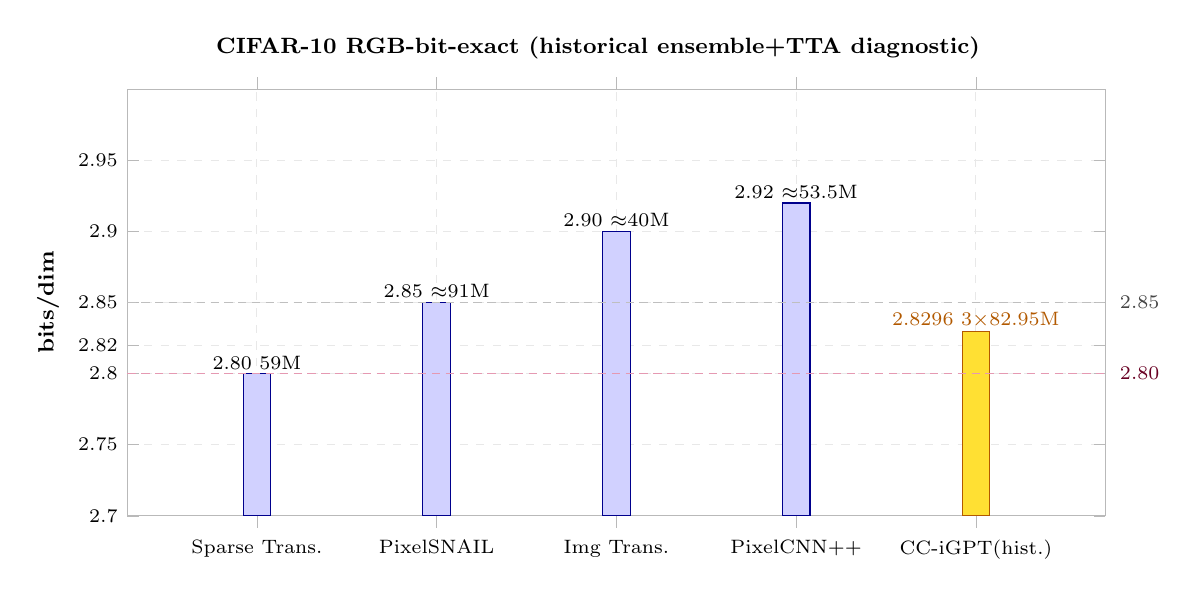
\begin{tikzpicture}[font=\footnotesize]
\begin{axis}[
    width=14cm, height=7cm,
    ybar,
    bar width=10pt,
    enlarge x limits=0.18,
    ymin=2.70, ymax=3.00,
    ytick={2.70,2.75,2.80,2.82,2.85,2.90,2.95},
    ylabel={\textbf{bits/dim}\ },
    ylabel near ticks,
    % 修复：明确指定所有5个x轴刻度，不再依赖xtick=data
    xtick={SparseTrans, PixelSNAIL, ImgTrans, PixelCNNpp, Ours},
    symbolic x coords={SparseTrans, PixelSNAIL, ImgTrans, PixelCNNpp, Ours},
    xticklabels={Sparse Trans., PixelSNAIL, Img Trans., PixelCNN++, CC-iGPT(hist.)},
    xticklabel style={font=\scriptsize, yshift=-1pt},
    yticklabel style={font=\scriptsize},
    axis line style={gray!55},
    tick style={gray!55},
    grid=major,
    grid style={dashed, gray!18, line width=0.3pt},
    major grid style={dashed, gray!18},
    clip=false,
]

% 前4个蓝色柱子（单独绘制，确保颜色正确）
\addplot[draw=blue!55!black, fill=blue!18, bar shift=0pt] coordinates {
    (SparseTrans, 2.80)
    (PixelSNAIL,  2.85)
    (ImgTrans,    2.90)
    (PixelCNNpp,  2.92)
};

% 第5个柔和橘黄色柱子（单独绘制，完全独立，不会被覆盖）
\addplot[draw=orange!70!black, fill=orange!30!yellow!80, bar shift=0pt] coordinates {
    (Ours, 2.8296)
};

% --- 参考线 1：PixelSNAIL 2.85；Ours 为不同成本、diagnostic protocol 下的历史实验，不作胜负结论 ---
\draw[densely dashed, gray!50, line width=0.4pt]
    ({rel axis cs:0,0}|-{axis cs:SparseTrans,2.85})
    -- ({rel axis cs:1,0}|-{axis cs:SparseTrans,2.85});
\node[font=\scriptsize, gray!55!black, anchor=west]
    at ({rel axis cs:1.005,0}|-{axis cs:SparseTrans,2.85}) {2.85};

% --- 参考线 2：Sparse Transformer 2.80 ---
\draw[densely dashed, purple!40, line width=0.4pt]
    ({rel axis cs:0,0}|-{axis cs:SparseTrans,2.80})
    -- ({rel axis cs:1,0}|-{axis cs:SparseTrans,2.80});
\node[font=\scriptsize, purple!55!black, anchor=west]
    at ({rel axis cs:1.005,0}|-{axis cs:SparseTrans,2.80}) {2.80};

% --- 手动标注bpd和参数量 ---
\node[font=\scriptsize, align=center, yshift=4pt] at (axis cs:SparseTrans, 2.80) {2.80 59M};
\node[font=\scriptsize, align=center, yshift=4pt] at (axis cs:PixelSNAIL, 2.85) {2.85 $\approx$91M};
\node[font=\scriptsize, align=center, yshift=4pt] at (axis cs:ImgTrans, 2.90) {2.90 $\approx$40M};
\node[font=\scriptsize, align=center, yshift=4pt] at (axis cs:PixelCNNpp, 2.92) {2.92 $\approx$53.5M};
\node[font=\scriptsize, align=center, orange!70!black, yshift=4pt] at (axis cs:Ours, 2.8296) {2.8296 $3{\times}$82.95M};

\end{axis}

% --- 标题 ---
\node[font=\footnotesize\bfseries, anchor=south, yshift=3pt]
    at (current bounding box.north) {CIFAR-10 RGB-bit-exact (historical ensemble+TTA diagnostic)};

\end{tikzpicture}
\end{document}

%
% 数据来源: README.md L27-35 (RGB-bit-exact 同域可比)
%   PixelCNN++         ~53.5M 2.92    Salimans et al., ICLR 2017  (公开 ~53.5M; 脚本核算锚 55.35M, 见 scripts/pixelsnail_paramcount.py)
%   Image Transformer  ~40M   2.90    Parmar et al., ICML 2018  (原文未报告参数量; ~40M 据官方 tensor2tensor imagetransformer_cifar10_base = 12L/d512/ff2048 估算)
%   PixelSNAIL         ~91M   2.85    Chen et al., ICML 2018  (原文未报告参数量; ~91M 据官方 neocxi/pixelsnail-public CIFAR 配置 h12_noup_smallkey/nr_filters=256/nr_resnet=4 核算, 见 scripts/pixelsnail_paramcount.py)
%   Sparse Transformer  59M   2.80    Child et al., 2019 (128 层 strided)
%   CC-iGPT v2 (historical experiment; diagnostic protocol) 3x82.95M 2.8296
%     R-only ensemble (best+SWA+EMA) + TTA hflip, 6 forwards/image；非正式单模型主表
\documentclass[tikz,border=8pt]{standalone}
\usepackage{tikz}
\usepackage{pgfplots}
\usepackage{amsmath,amssymb}
\pgfplotsset{compat=1.18}

\begin{document}
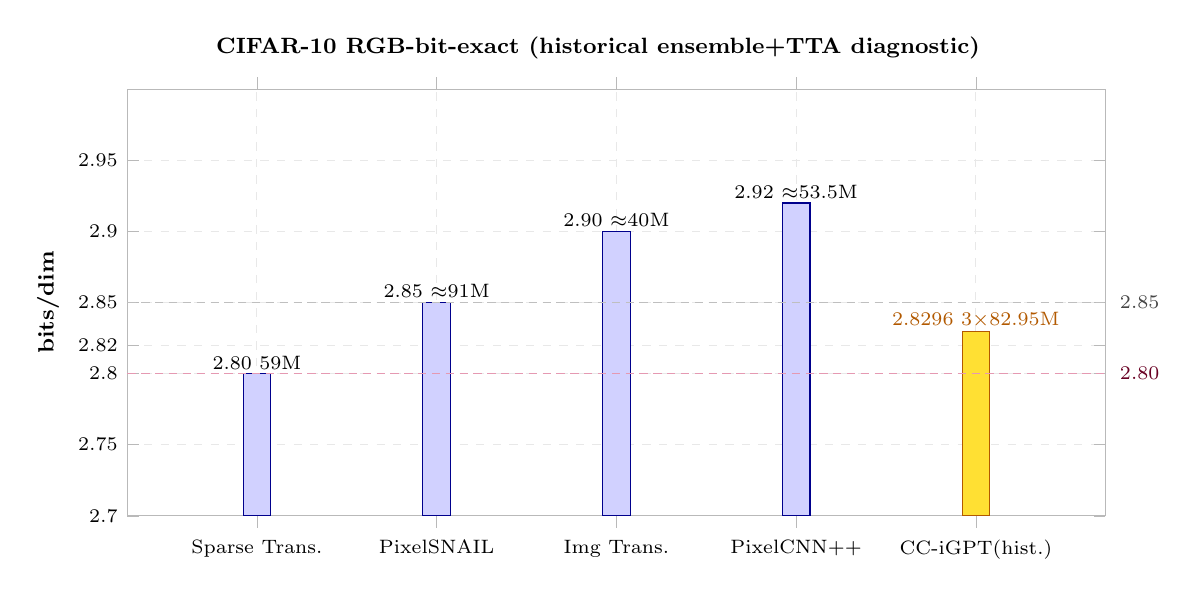
\begin{tikzpicture}[font=\footnotesize]
\begin{axis}[
    width=14cm, height=7cm,
    ybar,
    bar width=10pt,
    enlarge x limits=0.18,
    ymin=2.70, ymax=3.00,
    ytick={2.70,2.75,2.80,2.82,2.85,2.90,2.95},
    ylabel={\textbf{bits/dim}\ },
    ylabel near ticks,
    % 修复：明确指定所有5个x轴刻度，不再依赖xtick=data
    xtick={SparseTrans, PixelSNAIL, ImgTrans, PixelCNNpp, Ours},
    symbolic x coords={SparseTrans, PixelSNAIL, ImgTrans, PixelCNNpp, Ours},
    xticklabels={Sparse Trans., PixelSNAIL, Img Trans., PixelCNN++, CC-iGPT(hist.)},
    xticklabel style={font=\scriptsize, yshift=-1pt},
    yticklabel style={font=\scriptsize},
    axis line style={gray!55},
    tick style={gray!55},
    grid=major,
    grid style={dashed, gray!18, line width=0.3pt},
    major grid style={dashed, gray!18},
    clip=false,
]

% 前4个蓝色柱子（单独绘制，确保颜色正确）
\addplot[draw=blue!55!black, fill=blue!18, bar shift=0pt] coordinates {
    (SparseTrans, 2.80)
    (PixelSNAIL,  2.85)
    (ImgTrans,    2.90)
    (PixelCNNpp,  2.92)
};

% 第5个柔和橘黄色柱子（单独绘制，完全独立，不会被覆盖）
\addplot[draw=orange!70!black, fill=orange!30!yellow!80, bar shift=0pt] coordinates {
    (Ours, 2.8296)
};

% --- 参考线 1：PixelSNAIL 2.85；Ours 为不同成本、diagnostic protocol 下的历史实验，不作胜负结论 ---
\draw[densely dashed, gray!50, line width=0.4pt]
    ({rel axis cs:0,0}|-{axis cs:SparseTrans,2.85})
    -- ({rel axis cs:1,0}|-{axis cs:SparseTrans,2.85});
\node[font=\scriptsize, gray!55!black, anchor=west]
    at ({rel axis cs:1.005,0}|-{axis cs:SparseTrans,2.85}) {2.85};

% --- 参考线 2：Sparse Transformer 2.80 ---
\draw[densely dashed, purple!40, line width=0.4pt]
    ({rel axis cs:0,0}|-{axis cs:SparseTrans,2.80})
    -- ({rel axis cs:1,0}|-{axis cs:SparseTrans,2.80});
\node[font=\scriptsize, purple!55!black, anchor=west]
    at ({rel axis cs:1.005,0}|-{axis cs:SparseTrans,2.80}) {2.80};

% --- 手动标注bpd和参数量 ---
\node[font=\scriptsize, align=center, yshift=4pt] at (axis cs:SparseTrans, 2.80) {2.80 59M};
\node[font=\scriptsize, align=center, yshift=4pt] at (axis cs:PixelSNAIL, 2.85) {2.85 $\approx$91M};
\node[font=\scriptsize, align=center, yshift=4pt] at (axis cs:ImgTrans, 2.90) {2.90 $\approx$40M};
\node[font=\scriptsize, align=center, yshift=4pt] at (axis cs:PixelCNNpp, 2.92) {2.92 $\approx$53.5M};
\node[font=\scriptsize, align=center, orange!70!black, yshift=4pt] at (axis cs:Ours, 2.8296) {2.8296 $3{\times}$82.95M};

\end{axis}

% --- 标题 ---
\node[font=\footnotesize\bfseries, anchor=south, yshift=3pt]
    at (current bounding box.north) {CIFAR-10 RGB-bit-exact (historical ensemble+TTA diagnostic)};

\end{tikzpicture}
\end{document}

%
% 数据来源: README.md L27-35 (RGB-bit-exact 同域可比)
%   PixelCNN++         ~53.5M 2.92    Salimans et al., ICLR 2017  (公开 ~53.5M; 脚本核算锚 55.35M, 见 scripts/pixelsnail_paramcount.py)
%   Image Transformer  ~40M   2.90    Parmar et al., ICML 2018  (原文未报告参数量; ~40M 据官方 tensor2tensor imagetransformer_cifar10_base = 12L/d512/ff2048 估算)
%   PixelSNAIL         ~91M   2.85    Chen et al., ICML 2018  (原文未报告参数量; ~91M 据官方 neocxi/pixelsnail-public CIFAR 配置 h12_noup_smallkey/nr_filters=256/nr_resnet=4 核算, 见 scripts/pixelsnail_paramcount.py)
%   Sparse Transformer  59M   2.80    Child et al., 2019 (128 层 strided)
%   CC-iGPT v2 (historical experiment; diagnostic protocol) 3x82.95M 2.8296
%     R-only ensemble (best+SWA+EMA) + TTA hflip, 6 forwards/image；非正式单模型主表
\documentclass[tikz,border=8pt]{standalone}
\usepackage{tikz}
\usepackage{pgfplots}
\usepackage{amsmath,amssymb}
\pgfplotsset{compat=1.18}

\begin{document}
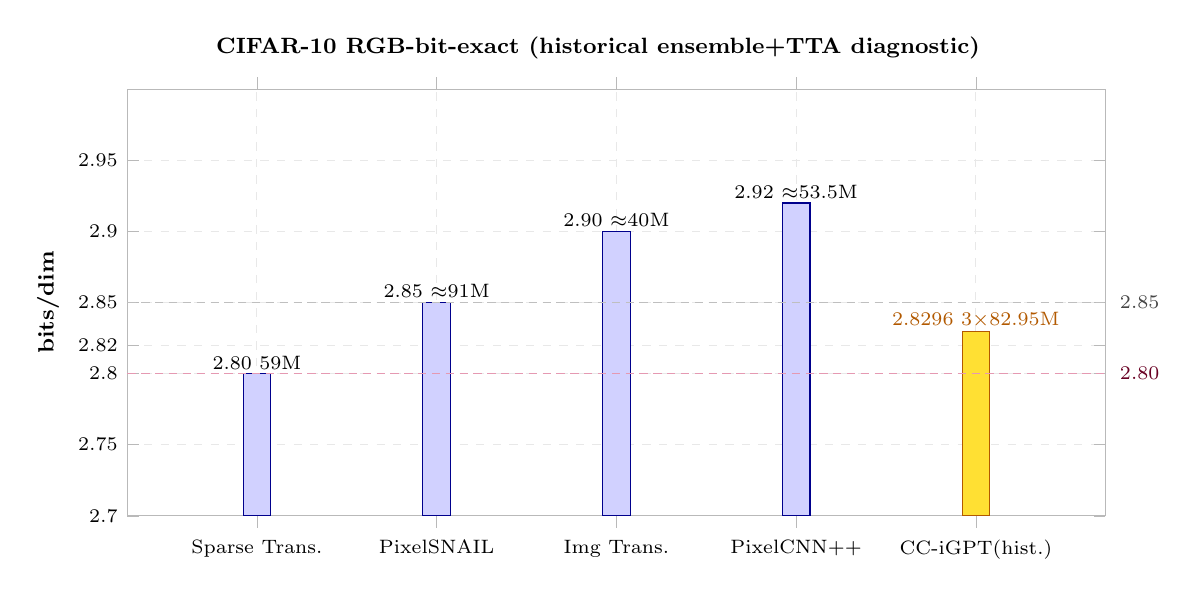
\begin{tikzpicture}[font=\footnotesize]
\begin{axis}[
    width=14cm, height=7cm,
    ybar,
    bar width=10pt,
    enlarge x limits=0.18,
    ymin=2.70, ymax=3.00,
    ytick={2.70,2.75,2.80,2.82,2.85,2.90,2.95},
    ylabel={\textbf{bits/dim}\ },
    ylabel near ticks,
    % 修复：明确指定所有5个x轴刻度，不再依赖xtick=data
    xtick={SparseTrans, PixelSNAIL, ImgTrans, PixelCNNpp, Ours},
    symbolic x coords={SparseTrans, PixelSNAIL, ImgTrans, PixelCNNpp, Ours},
    xticklabels={Sparse Trans., PixelSNAIL, Img Trans., PixelCNN++, CC-iGPT(hist.)},
    xticklabel style={font=\scriptsize, yshift=-1pt},
    yticklabel style={font=\scriptsize},
    axis line style={gray!55},
    tick style={gray!55},
    grid=major,
    grid style={dashed, gray!18, line width=0.3pt},
    major grid style={dashed, gray!18},
    clip=false,
]

% 前4个蓝色柱子（单独绘制，确保颜色正确）
\addplot[draw=blue!55!black, fill=blue!18, bar shift=0pt] coordinates {
    (SparseTrans, 2.80)
    (PixelSNAIL,  2.85)
    (ImgTrans,    2.90)
    (PixelCNNpp,  2.92)
};

% 第5个柔和橘黄色柱子（单独绘制，完全独立，不会被覆盖）
\addplot[draw=orange!70!black, fill=orange!30!yellow!80, bar shift=0pt] coordinates {
    (Ours, 2.8296)
};

% --- 参考线 1：PixelSNAIL 2.85；Ours 为不同成本、diagnostic protocol 下的历史实验，不作胜负结论 ---
\draw[densely dashed, gray!50, line width=0.4pt]
    ({rel axis cs:0,0}|-{axis cs:SparseTrans,2.85})
    -- ({rel axis cs:1,0}|-{axis cs:SparseTrans,2.85});
\node[font=\scriptsize, gray!55!black, anchor=west]
    at ({rel axis cs:1.005,0}|-{axis cs:SparseTrans,2.85}) {2.85};

% --- 参考线 2：Sparse Transformer 2.80 ---
\draw[densely dashed, purple!40, line width=0.4pt]
    ({rel axis cs:0,0}|-{axis cs:SparseTrans,2.80})
    -- ({rel axis cs:1,0}|-{axis cs:SparseTrans,2.80});
\node[font=\scriptsize, purple!55!black, anchor=west]
    at ({rel axis cs:1.005,0}|-{axis cs:SparseTrans,2.80}) {2.80};

% --- 手动标注bpd和参数量 ---
\node[font=\scriptsize, align=center, yshift=4pt] at (axis cs:SparseTrans, 2.80) {2.80 59M};
\node[font=\scriptsize, align=center, yshift=4pt] at (axis cs:PixelSNAIL, 2.85) {2.85 $\approx$91M};
\node[font=\scriptsize, align=center, yshift=4pt] at (axis cs:ImgTrans, 2.90) {2.90 $\approx$40M};
\node[font=\scriptsize, align=center, yshift=4pt] at (axis cs:PixelCNNpp, 2.92) {2.92 $\approx$53.5M};
\node[font=\scriptsize, align=center, orange!70!black, yshift=4pt] at (axis cs:Ours, 2.8296) {2.8296 $3{\times}$82.95M};

\end{axis}

% --- 标题 ---
\node[font=\footnotesize\bfseries, anchor=south, yshift=3pt]
    at (current bounding box.north) {CIFAR-10 RGB-bit-exact (historical ensemble+TTA diagnostic)};

\end{tikzpicture}
\end{document}

%
% 数据来源: README.md L27-35 (RGB-bit-exact 同域可比)
%   PixelCNN++         ~53.5M 2.92    Salimans et al., ICLR 2017  (公开 ~53.5M; 脚本核算锚 55.35M, 见 scripts/pixelsnail_paramcount.py)
%   Image Transformer  ~40M   2.90    Parmar et al., ICML 2018  (原文未报告参数量; ~40M 据官方 tensor2tensor imagetransformer_cifar10_base = 12L/d512/ff2048 估算)
%   PixelSNAIL         ~91M   2.85    Chen et al., ICML 2018  (原文未报告参数量; ~91M 据官方 neocxi/pixelsnail-public CIFAR 配置 h12_noup_smallkey/nr_filters=256/nr_resnet=4 核算, 见 scripts/pixelsnail_paramcount.py)
%   Sparse Transformer  59M   2.80    Child et al., 2019 (128 层 strided)
%   CC-iGPT v2 (historical experiment; diagnostic protocol) 3x82.95M 2.8296
%     R-only ensemble (best+SWA+EMA) + TTA hflip, 6 forwards/image；非正式单模型主表
\documentclass[tikz,border=8pt]{standalone}
\usepackage{tikz}
\usepackage{pgfplots}
\usepackage{amsmath,amssymb}
\pgfplotsset{compat=1.18}

\begin{document}
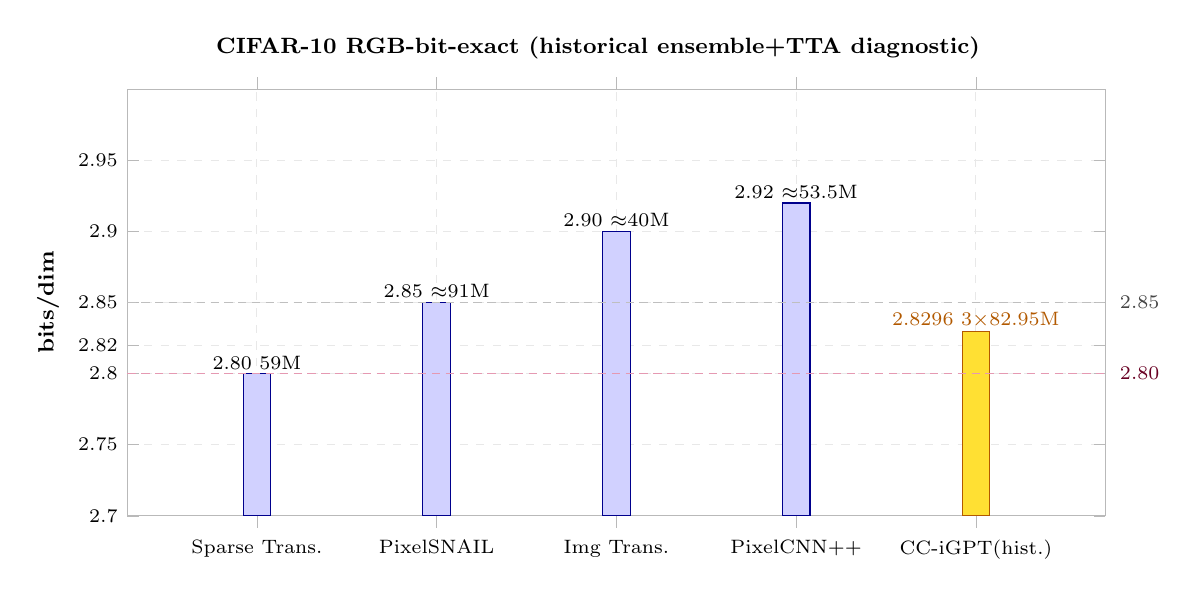
\begin{tikzpicture}[font=\footnotesize]
\begin{axis}[
    width=14cm, height=7cm,
    ybar,
    bar width=10pt,
    enlarge x limits=0.18,
    ymin=2.70, ymax=3.00,
    ytick={2.70,2.75,2.80,2.82,2.85,2.90,2.95},
    ylabel={\textbf{bits/dim}\ },
    ylabel near ticks,
    % 修复：明确指定所有5个x轴刻度，不再依赖xtick=data
    xtick={SparseTrans, PixelSNAIL, ImgTrans, PixelCNNpp, Ours},
    symbolic x coords={SparseTrans, PixelSNAIL, ImgTrans, PixelCNNpp, Ours},
    xticklabels={Sparse Trans., PixelSNAIL, Img Trans., PixelCNN++, CC-iGPT(hist.)},
    xticklabel style={font=\scriptsize, yshift=-1pt},
    yticklabel style={font=\scriptsize},
    axis line style={gray!55},
    tick style={gray!55},
    grid=major,
    grid style={dashed, gray!18, line width=0.3pt},
    major grid style={dashed, gray!18},
    clip=false,
]

% 前4个蓝色柱子（单独绘制，确保颜色正确）
\addplot[draw=blue!55!black, fill=blue!18, bar shift=0pt] coordinates {
    (SparseTrans, 2.80)
    (PixelSNAIL,  2.85)
    (ImgTrans,    2.90)
    (PixelCNNpp,  2.92)
};

% 第5个柔和橘黄色柱子（单独绘制，完全独立，不会被覆盖）
\addplot[draw=orange!70!black, fill=orange!30!yellow!80, bar shift=0pt] coordinates {
    (Ours, 2.8296)
};

% --- 参考线 1：PixelSNAIL 2.85；Ours 为不同成本、diagnostic protocol 下的历史实验，不作胜负结论 ---
\draw[densely dashed, gray!50, line width=0.4pt]
    ({rel axis cs:0,0}|-{axis cs:SparseTrans,2.85})
    -- ({rel axis cs:1,0}|-{axis cs:SparseTrans,2.85});
\node[font=\scriptsize, gray!55!black, anchor=west]
    at ({rel axis cs:1.005,0}|-{axis cs:SparseTrans,2.85}) {2.85};

% --- 参考线 2：Sparse Transformer 2.80 ---
\draw[densely dashed, purple!40, line width=0.4pt]
    ({rel axis cs:0,0}|-{axis cs:SparseTrans,2.80})
    -- ({rel axis cs:1,0}|-{axis cs:SparseTrans,2.80});
\node[font=\scriptsize, purple!55!black, anchor=west]
    at ({rel axis cs:1.005,0}|-{axis cs:SparseTrans,2.80}) {2.80};

% --- 手动标注bpd和参数量 ---
\node[font=\scriptsize, align=center, yshift=4pt] at (axis cs:SparseTrans, 2.80) {2.80 59M};
\node[font=\scriptsize, align=center, yshift=4pt] at (axis cs:PixelSNAIL, 2.85) {2.85 $\approx$91M};
\node[font=\scriptsize, align=center, yshift=4pt] at (axis cs:ImgTrans, 2.90) {2.90 $\approx$40M};
\node[font=\scriptsize, align=center, yshift=4pt] at (axis cs:PixelCNNpp, 2.92) {2.92 $\approx$53.5M};
\node[font=\scriptsize, align=center, orange!70!black, yshift=4pt] at (axis cs:Ours, 2.8296) {2.8296 $3{\times}$82.95M};

\end{axis}

% --- 标题 ---
\node[font=\footnotesize\bfseries, anchor=south, yshift=3pt]
    at (current bounding box.north) {CIFAR-10 RGB-bit-exact (historical ensemble+TTA diagnostic)};

\end{tikzpicture}
\end{document}
